\documentclass{article}
\usepackage[utf8]{inputenc}
\usepackage{graphicx}

\title{Membuat Aplikasi di Oracle Express Dengan Import Data Dari Excell}
\author{Helmi Azhar (1184013) }
\date{Oktober 2019}

\begin{document}

\maketitle

\section{Oracle express}
\begin{enumerate}
\usepackage{Oracle Apex merupakan suatu aplikasi atau tools  untuk memudahkan apa yang kita butuhkan. Sesuai namanya, oracle express bila dipelajari lebih dalam banyak memberi kemudahan dalam melayanani kebutuhan user contohnya dalam pembuatan aplikasi sederhana,belajar function dan lain-lain. Oracle apex juga dapat mengembangkan aplikasi web desktop dan seluler, memvisualisasikan dan memelihara data basis data, dan meningkatkan keterampilan sql dan kemampuan basis data}
\end{enumerate}

\begin{enumerate}
    \usepackage{pada tugas kali ini saya akan membuat aplikasi di oracle express dengan menginput data dari excell. sebagai contoh saya mengambil 50 data mahasiswa}
\end{enumerate}

\section{Langkah-langkah}
\begin{enumerate}
    \item sign in dengan akun masing-masing
    \begin{figure}
        \centering
        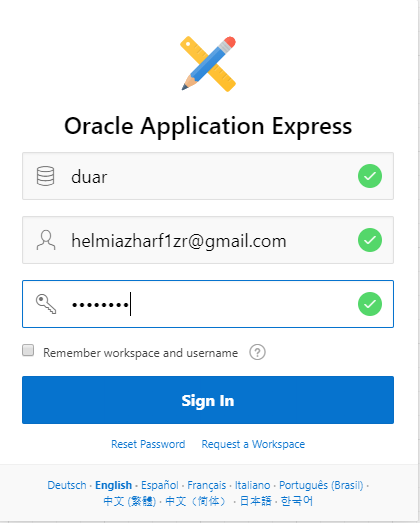
\includegraphics[scale=0.27]{gambar/1.PNG}
        \caption{Caption}
        \label{fig:my_label}
    \end{figure}

    \item setelah sign in pilih app builder
    \begin{figure}
        \centering
        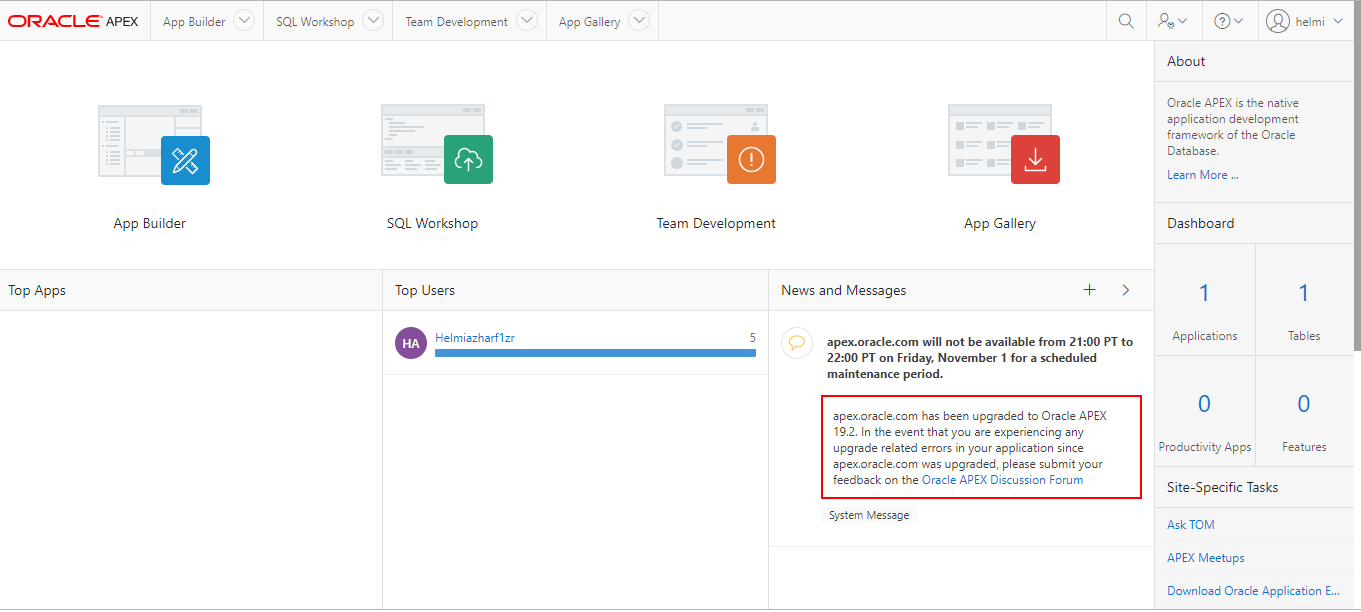
\includegraphics[scale=0.35]{gambar/2.PNG}
        \caption{Caption}
        \label{fig:my_label}
    \end{figure}

    \item buka create
    \begin{figure}
        \centering
        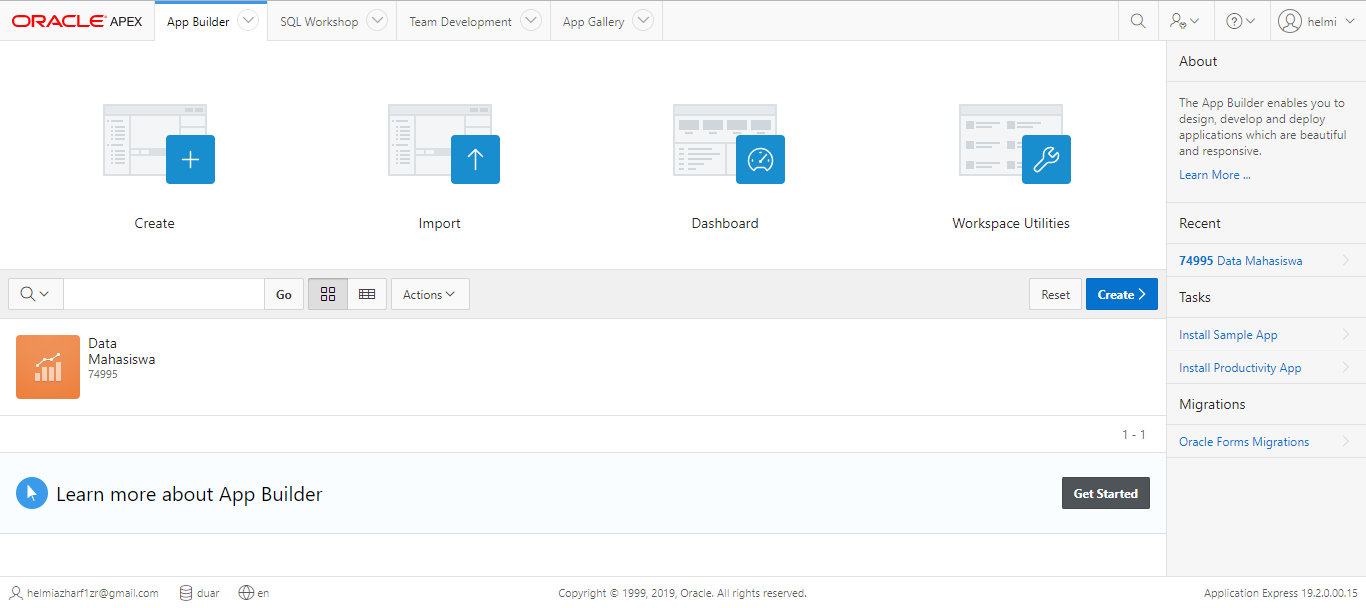
\includegraphics[scale=0.35]{gambar/3.PNG}
        \caption{Caption}
        \label{fig:my_label}
    \end{figure}

    \item lalu pilihm from a file
    \begin{figure}
        \centering
        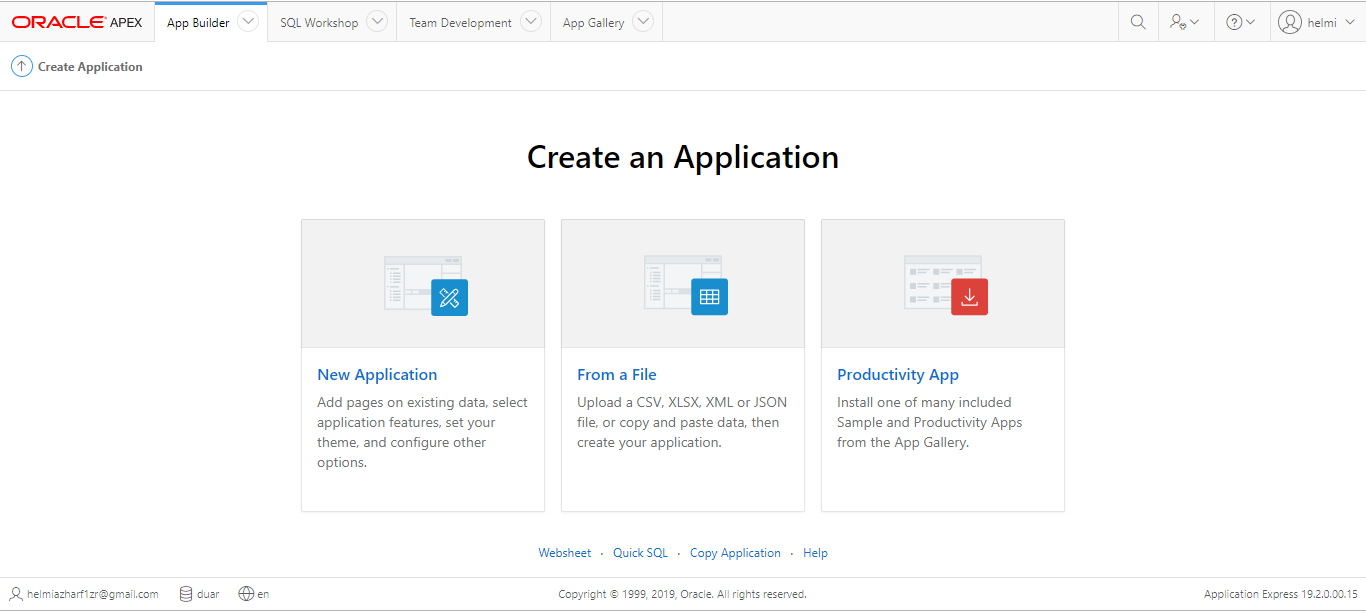
\includegraphics[scale=0.35]{gambar/4.PNG}
        \caption{Caption}
        \label{fig:my_label}
    \end{figure}

    \item pilih file yang akan di upload
    \begin{figure}
        \centering
        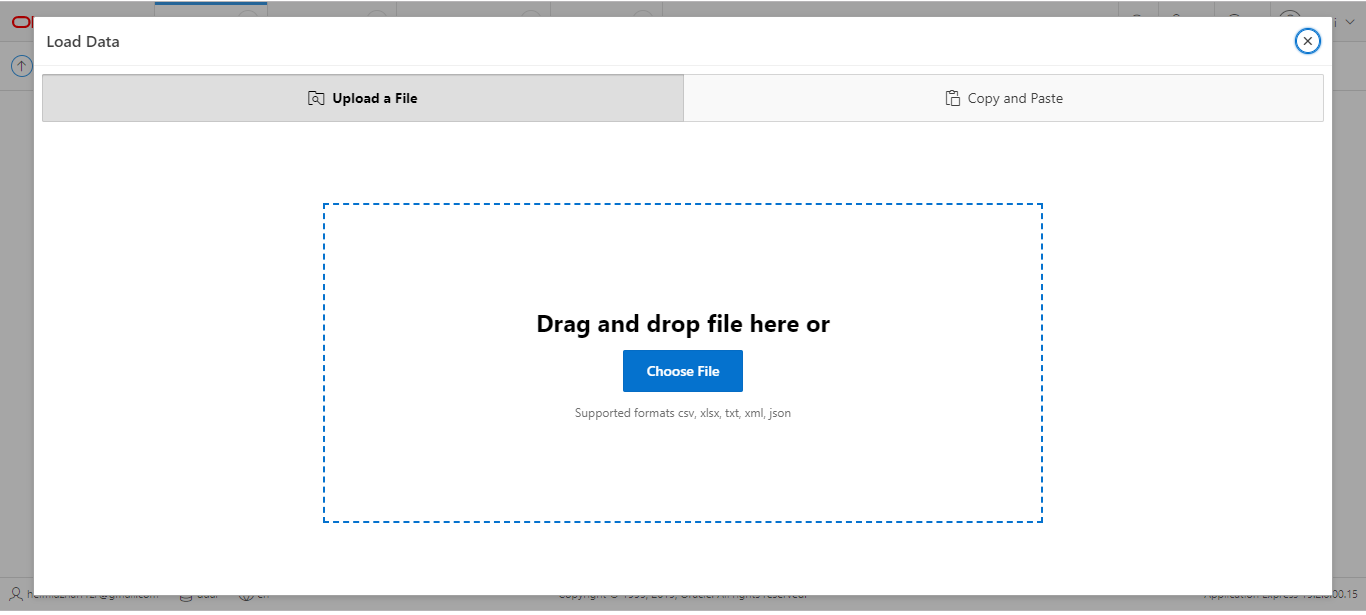
\includegraphics[scale=0.35]{gambar/5.PNG}
        \caption{Caption}
        \label{fig:my_label}
    \end{figure}

    \item isi nama tabel dan nama tabel error lalu load data dan create
    \begin{figure}
        \centering
        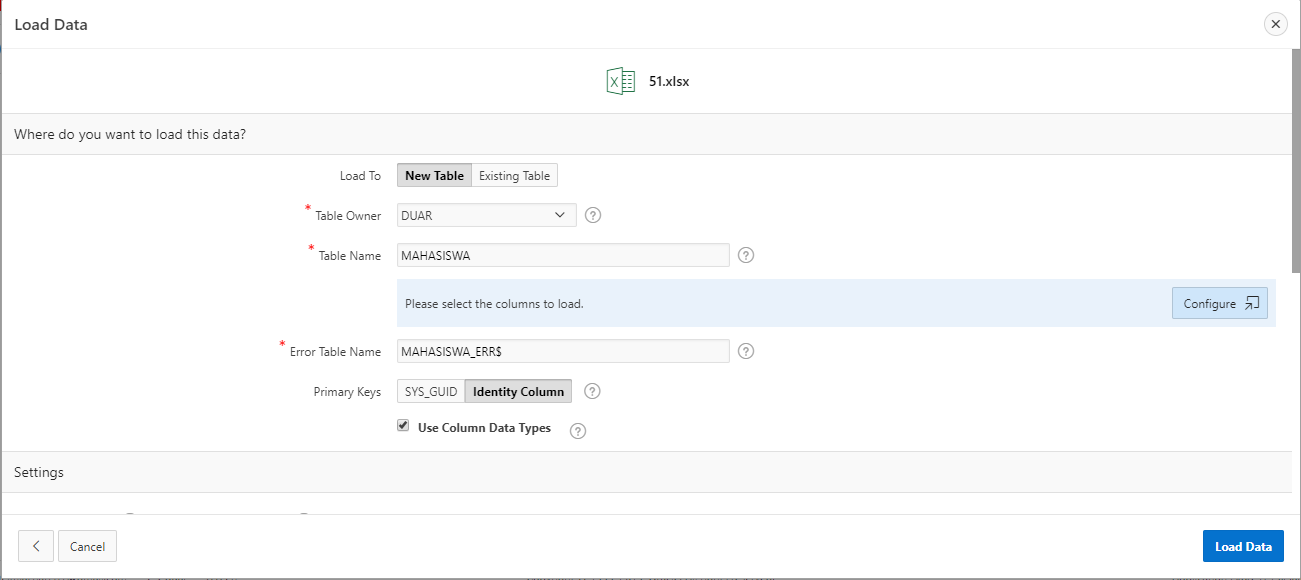
\includegraphics[scale=0.35]{gambar/6.PNG}
        \caption{Caption}
        \label{fig:my_label}
    \end{figure}
    
        \item apabila tampilan sudah seperti ini maka artinya data kita sudah masuk lalu buka run application untuk membuka data yang tadi
    \begin{figure}
        \centering
        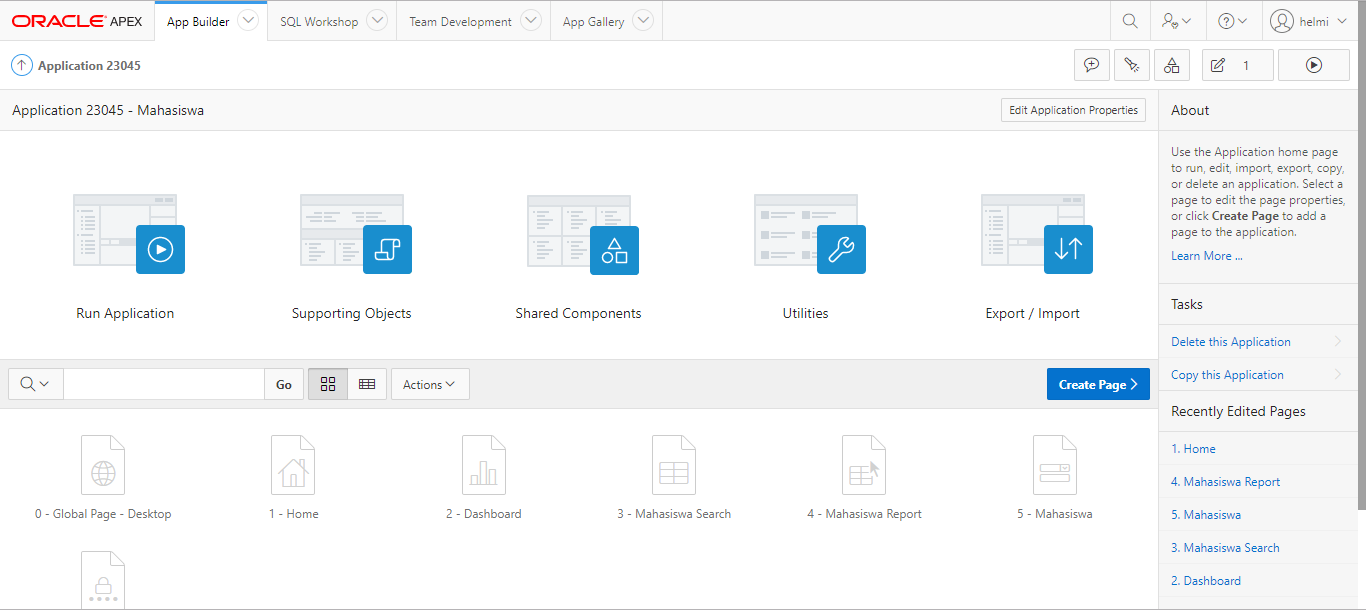
\includegraphics[scale=0.35]{gambar/7.PNG}
        \caption{Caption}
        \label{fig:my_label}
    \end{figure}
    
        \item sign in memakai akun kita
    \begin{figure}
        \centering
        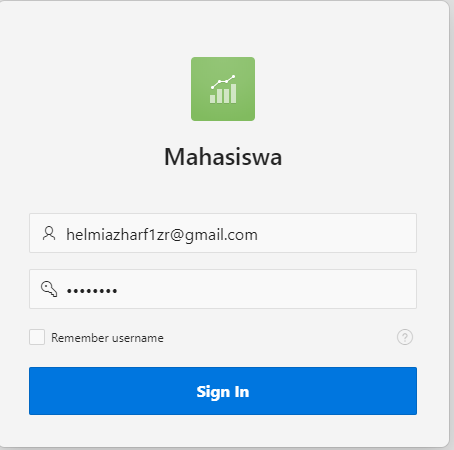
\includegraphics[scale=0.35]{gambar/8.PNG}
        \caption{Caption}
        \label{fig:my_label}
    \end{figure}
    
        \item pilih yang kita akan lakukan
    \begin{figure}
        \centering
        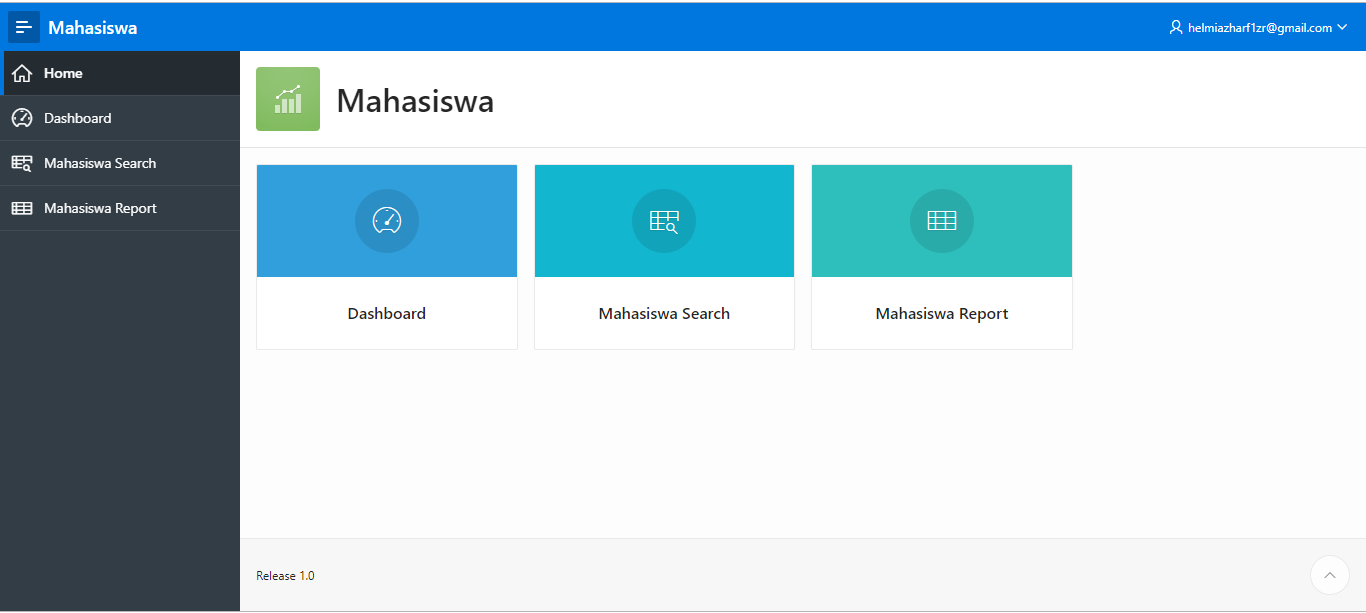
\includegraphics[scale=0.35]{gambar/9.PNG}
        \caption{Caption}
        \label{fig:my_label}
    \end{figure}
    \end{enumerate}
    
\section{Data Saya}
\begin{enumerate}
    \item workspace = "duar"
    \item username = "helmiazharf1zr@gmail.com"
    \item password = "password"
\end{enumerate}

    
\end{document}
